\documentclass[11pt,a4paper]{article}

\usepackage[T1]{fontenc}
\usepackage[utf8]{inputenc}
\usepackage[english]{babel}
\usepackage[a4paper,top=2.25cm,bottom=2.25cm,left=2.45cm,right=2.45cm,headsep=12pt]{geometry}
\usepackage{amsmath,amssymb,mathtools}
\usepackage{enumitem}
\usepackage{eurosym}
\usepackage{graphicx}
\usepackage{xcolor}
\usepackage{microtype}
\usepackage{avant}
\usepackage{mathptmx}
\usepackage{titlesec}
\usepackage{fancyhdr}
\usepackage{mdframed}
\usepackage{tikz}
\usepackage{needspace}
\usepackage{hyperref}
\usetikzlibrary{arrows.meta,positioning}

\definecolor{PPEBurgundy}{RGB}{112,28,47}
\definecolor{PPENavarraRed}{RGB}{211,32,46}
\definecolor{PPEGold}{RGB}{185,143,57}
\definecolor{PPEAccentLight}{RGB}{248,235,238}
\definecolor{PPEInk}{RGB}{37,31,33}
\definecolor{PPEMuted}{RGB}{101,83,88}

\hypersetup{colorlinks=true,linkcolor=PPEBurgundy,urlcolor=PPEBurgundy}
\setlength{\parindent}{0pt}
\setlength{\parskip}{0.42em}
\setlist[itemize]{topsep=0.25em,itemsep=0.18em,leftmargin=1.5em}
\setlist[enumerate]{topsep=0.3em,itemsep=0.35em,leftmargin=1.9em}
\raggedbottom
\allowdisplaybreaks[2]

\titleformat{\section}
  {\sffamily\bfseries\large\color{PPEInk}}
  {\color{PPEBurgundy}\thesection}{0.8em}{}
\titlespacing*{\section}{0pt}{1.1em}{0.45em}

\newmdenv[
  skipabove=0.55em,skipbelow=0.75em,
  leftline=true,rightline=false,topline=false,bottomline=false,
  linewidth=3pt,linecolor=PPEBurgundy,backgroundcolor=PPEAccentLight,
  innerleftmargin=0.75em,innerrightmargin=0.75em,
  innertopmargin=0.52em,innerbottommargin=0.52em
]{instructionsbox}

\pagestyle{fancy}
\fancyhf{}
\fancyhead[LE,LO]{\sffamily\small Microeconomics \textbar{} Midterm Examination \textbar{} Chapters 1--10}
\fancyhead[RE,RO]{\sffamily\small\color{PPEBurgundy}\thepage}
\fancyfoot[C]{\sffamily\scriptsize\color{PPEMuted}Politics, Philosophy and Economics \textbar{} University of Navarra}
\renewcommand{\headrulewidth}{0.45pt}
\renewcommand{\headrule}{\hbox to\headwidth{\color{PPEGold}\leaders\hrule height \headrulewidth\hfill}}
\setlength{\headheight}{15pt}

\newcommand{\answerline}{\rule{0.42\textwidth}{0.35pt}}
\newcommand{\shortblank}{\rule{0.17\textwidth}{0.35pt}}

\begin{document}

\begin{center}
  \IfFileExists{assets/branding/unav-logo-black.png}{%
    
\includegraphics[width=0.30\textwidth]{assets/branding/unav-logo-black.png}%
  }{%
    {\sffamily\bfseries\Large Universidad de Navarra}%
  }\par
  \vspace{0.5em}
  {\sffamily\color{PPENavarraRed}\large\textsc{Politics, Philosophy and Economics}\par}
  \vspace{0.3em}
  {\color{PPEGold}\rule{0.74\textwidth}{1.3pt}\par}
  \vspace{0.55em}
  {\sffamily\bfseries\color{PPEBurgundy}\LARGE Midterm Examination: Microeconomics\par}
  \vspace{0.16em}
  {\sffamily\large Chapters 1--10 \textbar{} 100 points\par}
\end{center}

\begin{instructionsbox}
\textbf{Instructions.} Answer all questions and show your work. For
computations, write the relevant formula, the algebra, and a brief economic
interpretation when requested. Draw labelled diagrams whenever asked. Unless a
question states otherwise, quantities are non-negative and continuously
divisible. No calculator is required or permitted.
\end{instructionsbox}

\textbf{Name and surname:} \rule{0.62\textwidth}{0.35pt}

\vspace{0.45em}
\section{Derivatives \hfill (6 points)}

Compute each derivative with respect to \(x\). When a function has other
variables, treat them as constants.

\begin{enumerate}[label=\textbf{\alph*.},itemsep=0.72em]
  \item \(f(x)=2x^2+6x+40\).
  \item \(g(x)=3x^4-4x^3+6x^2-8\).
  \item \(h(x)=f(x)g(x)=(2x^2+6x+40)(3x^4-4x^3+6x^2-8)\).
        Use the product rule; do not expand first.
  \item \(a(x)=[2x^2+6x+40]^{1/2}\). Use the chain rule.
  \item \(b(x)=[2x^2+6x+40]^{\beta}\), where \(\beta\) is a constant.
  \item \(i(x)=\dfrac{2x^2+6x}{x^3-4x}\). Use the quotient rule, or write
        the denominator with exponent \(-1\) and use the product and chain
        rules.
\end{enumerate}

\newpage
\section{Preference language and opportunity cost \hfill (14 points)}

\textbf{2. Translate into words. \hfill (4 points)}
\begin{enumerate}[label=\textbf{\alph*.}]
  \item \(A\sim B\).
  \item \(A\succ B\succeq C\).
\end{enumerate}

\vspace{0.3em}
\textbf{3. Use \(\sim\), \(\succ\), and \(\succeq\) to describe the
following comparisons. Assume monotonicity. \hfill (4 points)}

\begin{center}
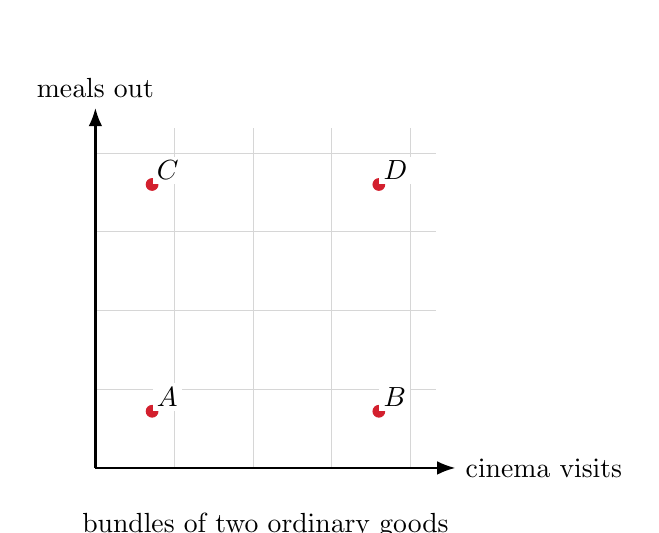
\begin{tikzpicture}[x=0.72cm,y=0.72cm,>=Latex]
  \draw[step=1cm,gray!32,very thin] (0,0) grid (6,6);
  \draw[->,thick] (0,0) -- (6.35,0) node[right] {cinema visits};
  \draw[->,thick] (0,0) -- (0,6.35) node[above] {meals out};
  \foreach \x/\y/\lab/\pos in {1/1/A/above right,5/1/B/above right,1/5/C/above right,5/5/D/above right}{
    \filldraw[PPENavarraRed] (\x,\y) circle (2.1pt);
    \node[\pos,fill=white,inner sep=1.5pt] at (\x,\y) {\(\lab\)};
  }
  \node[below] at (3,-0.62) {bundles of two ordinary goods};
\end{tikzpicture}
\end{center}

\begin{enumerate}[label=\textbf{\alph*.}]
  \item Compare \(A\) and \(B\).
  \item Compare \(A\) and \(C\).
  \item Compare \(A\) and \(D\).
  \item Compare \(C\) and \(B\).
\end{enumerate}

\vspace{0.2em}
\textbf{4.} A notebook costs \(\text{\euro}3\) and a textbook costs
\(\text{\euro}12\). What is the opportunity cost of one textbook measured in
notebooks? What is the opportunity cost of one notebook measured in textbooks?
\hfill (6 points)

\vfill
\newpage
\section{Consumer choice I \hfill (10 points)}

\textbf{5.} A student has a budget of \(\text{\euro}120\) to allocate between
two goods, \(x\) and \(y\). The price of \(x\) is \(\text{\euro}12\), the
price of \(y\) is \(\text{\euro}4\), and utility is \(u(x,y)=xy\).

\begin{enumerate}[label=\textbf{\alph*.}]
  \item Write the budget line and draw it. \hfill (2 points)
  \item Substitute the budget constraint into the utility function, so that
        utility depends only on \(x\). \hfill (1 point)
  \item Find the pair \((x,y)\) that maximises utility. Show the derivative
        and explain why the stationary point is a maximum. \hfill (7 points)
\end{enumerate}

\vspace{1.0em}
\begin{center}
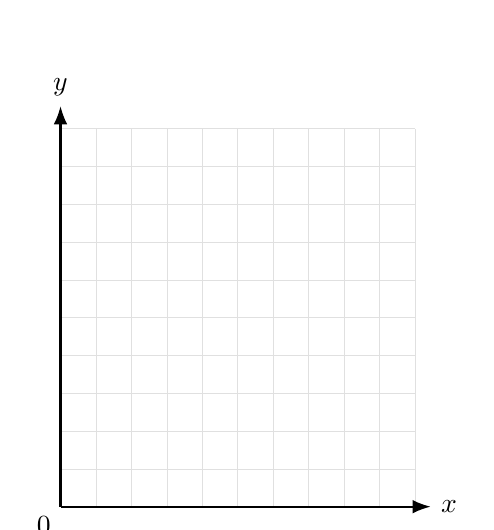
\begin{tikzpicture}[x=0.45cm,y=0.16cm,>=Latex]
  \foreach \x in {0,...,10}
    \draw[gray!24,very thin] (\x,0) -- (\x,30);
  \foreach \y in {0,3,...,30}
    \draw[gray!24,very thin] (0,\y) -- (10,\y);
  \draw[->,thick] (0,0) -- (10.45,0) node[right] {\(x\)};
  \draw[->,thick] (0,0) -- (0,31.8) node[above] {\(y\)};
  \node[below left] at (0,0) {\(0\)};
\end{tikzpicture}
\end{center}

\vfill
\newpage
\section{Consumer choice II \hfill (10 points)}

\textbf{6.} A consumer has a budget of \(\text{\euro}180\) and chooses between
goods \(x\) and \(y\). Prices are \(p_x=\text{\euro}20\) and
\(p_y=\text{\euro}10\). Preferences are represented by
\[
u(x,y)=x^{2/3}y^{1/3}.
\]

\begin{enumerate}[label=\textbf{\alph*.}]
  \item Write and draw the budget line. \hfill (2 points)
  \item Find the marginal rate of substitution \(\mathrm{MRS}_{x,y}\).
        \hfill (4 points)
  \item Use the tangency condition to find the optimal quantities of \(x\)
        and \(y\). \hfill (4 points)
\end{enumerate}

\vspace{1.0em}
\begin{center}
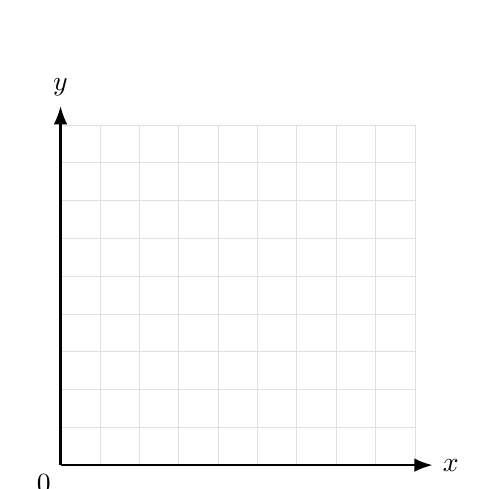
\begin{tikzpicture}[x=0.50cm,y=0.24cm,>=Latex]
  \foreach \x in {0,...,9}
    \draw[gray!24,very thin] (\x,0) -- (\x,18);
  \foreach \y in {0,2,...,18}
    \draw[gray!24,very thin] (0,\y) -- (9,\y);
  \draw[->,thick] (0,0) -- (9.45,0) node[right] {\(x\)};
  \draw[->,thick] (0,0) -- (0,19.0) node[above] {\(y\)};
  \node[below left] at (0,0) {\(0\)};
\end{tikzpicture}
\end{center}

\vfill
\newpage
\section{A price change: substitution and income effects \hfill (9 points)}

The diagram shows the choices of a consumer who buys coffee and sandwiches.
Initially, the budget line is \(RS\). The price of coffee then falls, so the
budget line pivots to \(RT\). The labelled indifference curves are
\(u_1\) and \(u_2\).

\begin{center}
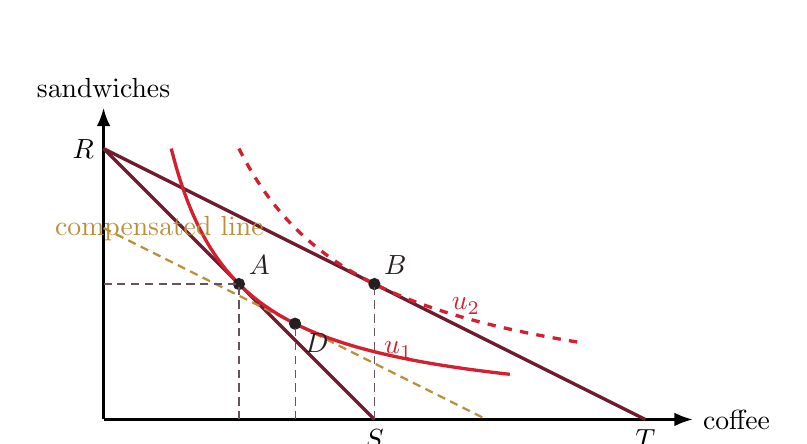
\begin{tikzpicture}[x=0.43cm,y=0.43cm,>=Latex]
  \draw[->,thick] (0,0) -- (17.4,0) node[right] {coffee};
  \draw[->,thick] (0,0) -- (0,9.2) node[above] {sandwiches};
  \coordinate (R) at (0,8);
  \coordinate (S) at (8,0);
  \coordinate (T) at (16,0);
  \draw[PPEBurgundy,very thick] (R) -- (S);
  \draw[PPEBurgundy,very thick] (R) -- (T);
  \draw[PPEGold,thick,densely dashed] (0,5.657) -- (11.314,0);
  \node[left] at (R) {\(R\)};
  \node[below] at (S) {\(S\)};
  \node[below] at (T) {\(T\)};
  \draw[PPENavarraRed,very thick,domain=2:12,samples=100,smooth]
    plot (\x,{16/\x});
  \draw[PPENavarraRed,very thick,dashed,domain=4:14,samples=100,smooth]
    plot (\x,{32/\x});
  \node[PPENavarraRed,right] at (8,2.05) {\(u_1\)};
  \node[PPENavarraRed,right] at (10,3.35) {\(u_2\)};
  \node[PPEGold,above] at (1.65,5.0) {compensated line};
  \filldraw[PPEInk] (4,4) circle (2pt) node[above right] {\(A\)};
  \filldraw[PPEInk] (5.657,2.828) circle (2pt) node[below right] {\(D\)};
  \filldraw[PPEInk] (8,4) circle (2pt) node[above right] {\(B\)};
  \draw[densely dashed,PPEMuted] (4,0) -- (4,4) -- (0,4);
  \draw[densely dashed,PPEMuted] (5.657,0) -- (5.657,2.828);
  \draw[densely dashed,PPEMuted] (8,0) -- (8,4);
\end{tikzpicture}
\end{center}

\begin{enumerate}[label=\textbf{\arabic*.},start=7]
  \item Before the price change, the consumer's optimum is point
        \shortblank. \hfill (2 points)
  \item After the price change, the consumer's optimum is point
        \shortblank. \hfill (2 points)
  \item The substitution effect moves demand from the original optimum to
        point \shortblank. \hfill (3 points)
  \item The income effect is the movement from point \shortblank\ to the new
        optimum. \hfill (2 points)
\end{enumerate}

\vfill
\newpage
\section{Cost curves and competitive supply \hfill (8 points)}

\textbf{11.} A price-taking firm sells reusable bottles at a market price of
\(\text{\euro}30\) per unit. Its total cost is
\[
TC(q)=36+6q+q^2.
\]
Answer the following questions.

\begin{enumerate}[label=\textbf{\alph*.}]
  \item What is fixed cost? \hfill (1 point)
  \item What are variable costs? \hfill (1 point)
  \item What is marginal cost? \hfill (1 point)
  \item What is average fixed cost? \hfill (1 point)
  \item What is average variable cost? \hfill (1 point)
  \item What quantity maximises profit? \hfill (1 point)
  \item At the profit-maximising quantity, what is average total cost?
        \hfill (1 point)
  \item At the profit-maximising quantity, what is marginal cost?
        \hfill (1 point)
\end{enumerate}

\vfill
\newpage
\section{Production and demand \hfill (15 points)}

\textbf{12.} A workshop has production function
\[
q=2L^{1/2}K^{1/2}.
\]
Calculate output when \(L=4\) and \(K=9\). If the workshop doubles both
inputs, by what factor does output change? Classify the returns to scale.
\hfill (3 points)

\vspace{0.6em}
\textbf{13.} Consider the inverse demand curve
\[
P=48-2Q.
\]
\begin{enumerate}[label=\textbf{\alph*.}]
  \item Calculate the price elasticity of demand using
        \(\varepsilon=(dQ/dP)(P/Q)\). \hfill (3 points)
  \item At what price and quantity is demand unit elastic?
        \hfill (2 points)
\end{enumerate}

\vspace{0.45em}
\textbf{14.} Total revenue on a linear demand curve is maximised where price
elasticity equals \answerline. \hfill (2 points)

\vspace{0.45em}
\textbf{15.} Demand for water at a beach kiosk is
\[
Q=120-2P.
\]
When \(P=\text{\euro}10\), a small increase in price will
\answerline\ total revenue. Explain briefly. \hfill (3 points)

\vspace{0.45em}
\textbf{16.} Is the cross-price elasticity of demand for substitute goods
positive or negative? \hfill (2 points)

\vfill
\newpage
\section{Elasticity and rational preferences \hfill (8 points)}

\textbf{17.} A 20\% fall in the price of rice leads to a 10\% increase in the
quantity demanded of rice and a 5\% fall in the quantity demanded of pasta.

\begin{enumerate}[label=\textbf{\alph*.}]
  \item What is the own-price elasticity of demand for rice? \hfill (1 point)
  \item What is the cross-price elasticity of demand between rice and pasta?
        \hfill (1 point)
  \item Rice and pasta are \answerline\ because the cross-price elasticity is
        \answerline. \hfill (1 point)
\end{enumerate}

\vspace{0.7em}
\textbf{18.} If the absolute value of the own-price elasticity of demand is
\(0.5\), what percentage change in quantity demanded follows from a 10\%
increase in price? State the direction of the change. \hfill (2 points)

\vspace{0.7em}
\textbf{19.} State three standard conditions used to describe rational
preferences. \hfill (3 points)

\vfill
\newpage
\section{Profit maximisation \hfill (5 points)}

\textbf{20.} A competitive firm sells sandwiches at a market price of
\(\text{\euro}20\). Its total cost is
\[
TC(q)=30+4q+q^2.
\]
\begin{enumerate}[label=\textbf{\alph*.}]
  \item Write the profit function. \hfill (2 points)
  \item Maximise profit. \hfill (2 points)
  \item Calculate profit at the optimal quantity. \hfill (1 point)
\end{enumerate}

\vfill
\newpage
\section{Key concepts \hfill (15 points)}

\textbf{21. Define each term or concept in one or two precise sentences.}
\hfill (1 point each)

\begin{enumerate}[label=\textbf{\alph*.},itemsep=0.62em]
  \item Economics
  \item Opportunity cost
  \item Marginal analysis
  \item Preference
  \item Indifference curve
  \item Marginal rate of substitution
  \item Budget set
  \item Normal good
  \item Price elasticity of demand
  \item Cross-price elasticity of demand
  \item Production function
  \item Marginal product
  \item Fixed cost
  \item Variable cost
  \item Marginal cost
\end{enumerate}

\end{document}

